Osserviamo l'andamento di alcune quantità che dipendono dal riempimento con elettroni dei livelli di un atomo.

\subsection{Raggio atomico}

Questa grandezza è in teoria infinita, ma abbiamo deciso di assegnare un raggio ad ogni atomo e dire che il nucleo è sostanzialmente piccolissimo e le dimensioni dell'atomo sono dovute agli orbitali, quindi agli elettroni (in particolar modo a quelli più esterni, che poi sono quelli di valenza). Stiamo inoltre imponendo che la probabilità di trovare l'elettrone sia confinata entro un certo valore che riteniamo accettabile. Fare questo ragionamento ha senso, perché nell'istante in cui avessi una molecola, se essa è formata da due atomi a raggi infiniti, quale sarebbe la distanza di legame tra i due atomi? Sarebbe infinita, ma ciò non è vero, perché noi siamo in grado di misurare le distanze nucleari e le distanze interatomiche nelle molecole. Quindi l'assunzione di confinare le dimensioni dei raggi degli atomi e degli ioni ragionando sul concetto probabilistico è indispensabile, ed è ciò che i parametri metrici delle molecole ci suggeriscono, ossia possiamo fare misure di distanze interatomiche sia in solidi che in sistemi molecolari gassosi, e pertanto l'avere pensato che gli ioni abbiano dimensioni ben precise è più che ragionevole.\\

Si osserva che i raggi degli atomi crescono all'aumentare del numero quantico principale n, in quanto l'energia dell'elettrone cresce in valore assoluto e dunque aumenta la distanza elettrone-nucleo. Quindi scendendo lungo un gruppo il raggio atomico aumenta.


Alcuni elementi non rispettano questa regola, come ad esempio il gallio, la cui anomalia è causata dal fatto che esso è un metallo allo stato liquido, per cui entrano in gioco altri fattori.\\

Lungo i periodi invece si nota esattamente il contrario: le dimensioni dell'atomo diminuiscono. Il motivo è che a differenza dei gruppi dove il fattore preponderante è n, qui lo è l'aumento di carica nucleare. Se la carica nucleare aumenta, ma n rimane uguale, gli elettroni si schermano poco reciprocamente e quindi l'aumento di carica nucleare fa si che le dimensioni dell'atomo diminuiscano.

Andando un gruppo succede l'esatto contrario: i livelli interni schermano molto gli elettroni esterni dalla carica nucleare, per cui questi ultimi non la sentono tutta ma solo una parte, col risultato di essere meno legati e quindi più distanti dal nucleo.

\begin{figure}[htp]
    \centering
    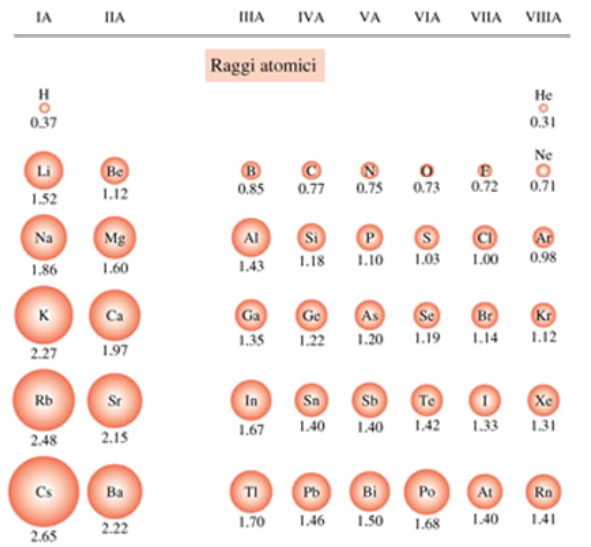
\includegraphics[width=12cm]{immagini/raggi-atomici.png}
\end{figure}

Quindi la carica nucleare:
\begin{itemize}
    \item Si sente molto lungo un periodo perché gli elettroni a parità di n si schermano poco reciprocamente.
    \item Si sente meno lungo un gruppo perché i livelli interni sono pieni (quando si arriva al gas nobile abbiamo riempito tutti i livelli interni), gli elettroni al loro interno schermano tantissimo quelli esterni dalla carica nucleare.
\end{itemize}
\subsection{Raggio degli ioni}
Quanto osservato per i raggi atomici in larga misura vale anche per i raggi degli ioni: crescono lungo un gruppo perché cresce il valore di n, mentre per quello che succede lungo un periodo bisogna ragionare in termini di stato d'ossidazione dato che abbiamo a che fare con ioni, e non ha senso confrontare ad esempio uno ione +1 con uno +2 o +3, dobbiamo confrontare ioni con la stessa carica. Infatti non avrebbe senso confrontare ad esempio l'\ce{N^{3-}} con l'N: il primo ha acquistato elettroni, e risulta quindi più grande.

Quindi quando si va lungo un periodo, per i raggi ionici bisogna fare ragionamenti che tengano conto della carica, mentre per un gruppo il ragionamento è più immediato: lungo esso le dimensioni aumentano così come aumentavano per gli atomi, perché all'interno di un gruppo si ha la stessa carica (Es 1° gruppo $\rightarrow$ un solo elettrone esterno. Se diventano ioni hanno tutti perso l'unico elettrone esterno, quindi sono tutti nella stessa situazione, avranno la configurazione elettronica del gas nobile che li precede, perché avevano un elettrone 2s, 3s, 4s ecc. da atomo, lo hanno perso e quindi hanno acquisito la configurazione dell'atomo che li precede, simile al gas nobile. Quindi ciò che osservo nel gas nobile lo riosservo nella sequenza. Analogamente si ragiona per gli elementi del secondo gruppo se perdono 2 elettroni, i quali avranno configurazione elettronica del gas nobile che li precede. Infine per gli elementi del terzo gruppo, se hanno stato di ossidazione +3 devo osservare lo stesso fenomeno. Se invece lo stato di ossidazione cambia la situazione si complica). Quindi quando si parla di raggi ionici si devono confrontare ioni con la stessa carica.

\begin{figure}[htp]
    \centering
    \includegraphics[width=12cm]{immagini/raggi-ionici.png}
\end{figure}

I lantanidi sono elettroluminescenti, infatti gli schermi, i display, sono costruiti con essi.

In essi si osserva che la dimensione dell'atomo diminuisce man mano che si va lungo la serie. Si parla dunque di "\textbf{contrazione lantanidica}", perché interviene un effetto relativistico: la massa di un elettrone aumenta all'aumentare della sua velocità, man mano che si avvicina alla velocità della luce. Gli elettroni s e p degli elementi "pesanti" hanno aumenti di massa fino al 20\%. Il raggio di un atomo è inversamente proporzionale alla massa di un elettrone.
\subsection{Potenziale di ionizzazione}
Quando due elementi o due composti reagiscono tra loro, ciò che avviene è uno scambio di elettroni (scambio non significa cessione totale, ma in qualche modo c'è una messa in comune, una condivisione di elettroni, ossia cambia l'assetto elettronico degli atomi, si ha una struttura elettronica diversa, pertanto l'idea di perdere o di acquistare elettroni sono due situazioni limite valide solo per sistemi puramente ionici. Ciò è da tenere a mente perché se un elemento ha i suoi elettroni esterni fortemente legati sarà poco reattivo, se si verifica il contrario sarà propenso a reagire.).

In generale con potenziale di ionizzazione indichiamo l'idea concettuale di Einstein: l'energia necessaria per far si che l'elettrone vinca l'attrazione elettrone-nucleo.\\

Oggi misurare il potenziale di ionizzazione è semplice: si strappano gli elettroni e si verifica l'energia richiesta, così da costruire la configurazione elettronica in funzione delle varie energie richieste.

Ragioniamo sull'aspetto formale di questo fenomeno: immaginiamo di avere un elemento e vogliamo che esso sia libero, cioè non abbia costrizioni di natura geometrica dovute ad un eventuale solido nel quale esso si trovi, in altre parole consideriamo atomi gassosi in sistemi rarefatti, in modo tale che il generico atomo o molecola sia effettivamente immaginabile come isolato e quindi non sottoposto ad alcun'altra interazione. A quest'atomo inviamo un'energia $h\nu$, e se è sufficiente l'atomo espellerà un elettrone e si caricherà positivamente perché avrà un eccesso di carica positiva:

$$\ce{M ->[$h\nu$] M+ + e-} \qquad \text{Potenziale di prima ionizzazione} \; \ce{(PI_1)}$$
È chiaro che \ce{M+} ha un tempo di vita molto piccolo ed è difficile studiarlo perché è difficile fare misure con un tempo di vita basso, pertanto la probabilità che si abbia una seconda ionizzazione, ossia che inviando un'alta energia questa ionizzi \ce{M+} ad \ce{M^{2+}} è scarsa, ma supponendo che avvenga chiameremo l'energia necessaria potenziale di seconda ionizzazione \ce{PI_2}
$$\ce{M+ -> M^{2+} + e-}$$
E così a crescere: terza, quarta ecc.

Da notare che nei composti è più facile da ottenere una seconda ionizzazione, infatti si conoscono alcuni di questi che cedono anche 3 elettroni (soprattutto nei composti ionici).

\textbf{ES 1}\\

\begin{tabular}{ m{4cm} m{4cm} }
\ce{Li -> Li+ + e-} & \ce{PI_1}\text{=5.39 eV} \\ 
\ce{Li+ -> Li^{2+} + e-} & \ce{PI_2}\text{=50.0 eV}  \\  
\ce{Li^{2+} -> Li^{3+} + e-} & \ce{PI_3}\text{=122.4 eV}
\end{tabular}\\

Il litio sta sotto l'idrogeno, quindi ha gli orbitali 1s totalmente pieni, e un terzo elettrone nell'orbitale 2s, quindi se volessi strappargli questo elettrone esterno, avrei:
$$\ce{Li_{gassoso} ->[$+h\nu$] Li+ + e-}$$
L'energia richiesta non è elevatissima. Lo ione \ce{Li+} avrà la configurazione elettronica dell'elio.

Se volessimo strappare un secondo elettrone al litio, stavolta dovremmo prenderlo dal livello 1s, a numero quantico inferiore, mentre il primo stava nel 2s, che è un orbitale di valenza perché è il più esterno, a numero quantico massimo per il litio. L'orbitale 1s è estremamente più vicino al nucleo, e il valore del potenziale di ionizzazione cambia drasticamente. Ciò dipende dal fatto che non sto strappando più elettroni di valenza ma "elettroni di core", interni, ad un livello a numero quantico inferiore.

Se volessi strappare anche il terzo ed ultimo elettrone del litio, l'energia richiesta aumenta ulteriormente.

È quindi ragionevole pensare che, nei suoi composti, la reattività del litio sia confinata all'esistenza dello ione \ce{Li+}, cioè nelle reazioni chimiche lavoriamo con gli elettroni di valenza, non riusciremo mai a coinvolgere così attivamente gli elettroni interni: essi sentiranno l'intorno chimico, ma non avremo stati di ossiazione che dipendono dal mettere in gioco anche elettroni a numero quantico inferiore, ossia elettroni interni.

\textbf{ES 2}\\

\begin{tabular}{ m{4cm} m{4cm} }
 \ce{Na -> Na+ + e-} & \ce{PI_1}\text{=5.12 eV} \\ 
 \ce{Na+ -> Na^{2+} + e-} & \ce{PI_2}\text{=47.05 eV}  \\  
 \ce{Na^{2+} -> Na^{3+} + e-} & \ce{PI_3}\text{=70.70 eV}
\end{tabular}\\

Il sodio sta sotto al litio, quindi ha esattamente la stessa configurazione elettronica esterna, con la differenza che il singolo elettrone esterno sta nell'orbitale 3s invece del 2s. Quindi l'energia di prima ionizzazione del sodio è minore di quella del litio perché questo elettrone è più esterno. Na$^+$ ha la configurazione elettronica del gas nobile che lo precede, il neon. Se volessi strappare il secondo elettrone al sodio Na$^+$, dovrei strappare elettroni appartenenti ad un orbitale relativo ad un numero quantico inferiore e l'energia di ionizzazione aumenterebbe, stessa cosa per un terzo elettrone. 

Risulta chiaro che, quando c'è un salto di numero quantico principale, le energie in gioco cambiano drasticamente e quando si fa reattività chimica si lavora sempre ed esclusivamente con gli elettroni di valenza, cioè quelli più esterni.\\

Osserviamo ora come vari, atomo per atomo, il potenziale di ionizzazione:

\begin{figure}[htp]
    \centering
    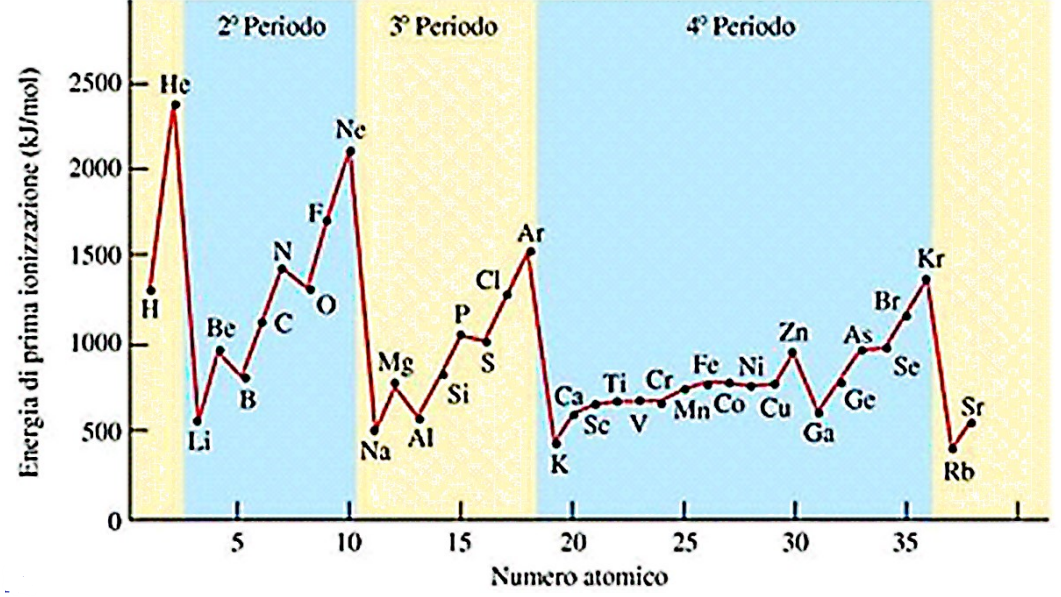
\includegraphics[width=12cm]{immagini/potenziale-di-ionizzazione.png}
\end{figure}

\begin{itemize}
    \item L'idrogeno ha potenziale di prima ionizzazione di circa 1500  kJ/mol.
    \item L'elio richiede circa 2400 kJ/mol perché è aumentata di una unità il suo numero atomico (due protoni invece di uno che attraggono gli elettroni) per cui, pur essendo 2 gli elettroni 1s, si ha un aumento in energia.
    \item Il litio richiede circa 500 kJ/mol: l'energia richiesta crolla perché l'elettrone da ionizzare sta nell'orbitale 2s e gli elettroni nell'orbitale 1s schermano l'elettrone più esterno (nel 2s) dalla carica nucleare.
    \item Il berillio richiede invece più energia perché aumenta di una unità la carica nucleare ma l'elettrone più esterno si trova comunque nell'orbitale 2s, cioè stesso numero quantico principale del litio. 
    \item Il boro richiede meno energia del berillio perché l'elettrone più esterno si trova nel 2p che è ancora meno legato del 2s.
    \item Per il carbonio serve più energia perché, nonostante l'elettrone più esterno si trovi nel 2p, la sua carica nucleare è aumentata.
    \item Analogamente per l'azoto perché gli orbitali 2p sono 3 e quindi col boro, carbonio e azoto si riempiono con un elettrone per orbitale con spin paralleli.
    \item Per l'ossigeno serve meno energia perché esso ha 4 elettroni negli orbitali 2p, per cui il quarto elettrone si posiziona in un orbitale che era già parzialmente occupato. Quindi un orbitale ha due elettroni, ma l'avere due elettroni nello stesso orbitale destabilizza il sistema perché i due elettroni si respingono (elettricamente): la repulsione tra i due elettroni fa si che serva meno energia per ionizzare l'atomo.
    \item Per il fluoro nonostante riempiamo con un ulteriore elettrone (sono 5) gli orbitali p, la carica nucleare aumenta ed il suo effetto si sente di più, per cui è richiesta più energia.
    \item Per il neon questo effetto culmina perché si riempiono tutti gli orbitali p ma l'aumento di carica nucleare mi determina l'aumento, da ossigeno, fluoro a neon, del potenziale di ionizzazione.
\end{itemize}
Quanto detto si generalizza per ciascun periodo della tavola periodica.
I valori maggiori di potenziali osservati sono quelli dei gas nobili: elio e neon. Dopo il neon crolla nuovamente il potenziale richiesto per ionizzare l'unico elettrone esterno del sodio, che sta nel 3s. Sebbene sia aumentata la carica nucleare, è aumentato pure il numero quantico principale e dunque l'elettrone è più esterno. Poi, come abbiamo visto per il berillio, osserviamo un aumento pure per il magnesio perché aumenta la carica nucleare. In seguito come per il boro l'energia di ionizzazione dell'alluminio diminuisce perché è il primo elemento del terzo periodo a contenere elettroni p. Poi come per il carbonio e azoto, l'energia sale per silicio e fosforo. Poi con lo zolfo scende come per l'ossigeno. Con zolfo, cloro e argon va a risalire come con ossigeno, fluoro e neon. Anche qui il valore più alto di energia è osservato per l'argon, un altro gas nobile, e così come per il litio osservavo il valore inferiore di energia di ionizzazione, noto che il sodio, che sta sotto il litio (che ha quindi stessa configurazione elettronica esterna), ha la minore energia di ionizzazione. E tutto si ripete partendo dal potassio.
Quindi questo trend, che cambia con gli elementi di transizione, è generico ed è ragionevole averlo interpretato conoscendo le loro strutture elettroniche, ossia ci siamo accorti che semplici considerazioni che derivano dall'aver imparato quali siano le strutture elettroniche di questi atomi ci permettono di ragionare e razionalizzare le \textbf{proprietà periodiche}: raggio atomico, raggio ionico e potenziale di prima ionizzazione. 
Qui non c'è reattività chimica coinvolta, ma essa è tutta derivabile dale strutture elettroniche dei sistemi interagenti, cioè in base al riempimento degli orbitali.
\subsection{Affinità elettronica}
L'affinità elettronica è un'altra proprietà che spieghiamo mediante le strutture elettroniche. È il contrario del potenziale di ionizzazione: col potenziale di ionizzazione inviamo energia per strappar elettroni, mentre con l'affinità elettronica diamo elettroni al sistema, il quale cede energia (nella maggior parte dei casi). Si parla quindi di energia liberata. Secondo la convezione termodinamica infatti, se un sistema acquista energia il $\Delta$H è positivo, se cede energia all'ambiente circostante è negativo. 

\textbf{ES}
$$\ce{ F^- -> F + e^-}\quad \text{PI} = 85\,\,\frac{\text{kcal}}{\text{mol}}=3.45 \text{ eV}$$
Il potenziale di ionizzazione è positivo perché noi diamo energia ad un sistema per strappargli un elettrone.
$$\ce{ F + e^- -> F^-}\quad \text{A} =-85\,\,\frac{\text{kcal}}{\text{mol}}=-3.45 \text{ eV}$$
L'affinità elettronica è negativa: il sistema si stabilizza quando acquista l'elettrone e quindi cede energia.

\textbf{DEF} Affinità elettronica: è l'energia (di norma) liberata quando si forma uno ione negativo:
$$\ce{ A + e- -> A-}$$ 
Riprendiamo l'esempio del fluoro: cedendogli un elettrone otteniamo uno ione negativo e la liberazione di energia. Si osserva che il potenziale di ionizzazione definito per l'anione è il fenomeno inverso, ossia se volessimo strappare un elettrone a F$^-$ e farlo ridiventare fluoro neutro atomco, l'energia richiesta sarebbe la stessa di quella ceduta ma cambiata di segno. Quindi per l'anione, l'affinità elettronica corrisponde al suo potenziale di ionizzazione.

Scendendo lungo un gruppo il valore di affinità elettronica diminuisce, cioè diventa meno negativo, mentre lungo un periodo diventa più negativo.
\begin{center}
    \begin{tabular}{ m{1cm}|m{2cm} } 
     F & -3.45 eV \\ 
     \hline
     Cl & -3.61 eV \\
     \hline
     Br & -3.36 eV \\ 
     \hline
     I & -3.06 eV \\
     \hline
    \end{tabular}
    \end{center}
Fluoro, cloro, bromo e iodio sono tutti alogeni, fanno quindi parte dello stesso gruppo. Per tutti eccetto il fluoro, si osserva che il valore di affinità elettronica diminuisce. Il motivo per cui il fluoro fa eccezione è perché lo ione fluoruro è piccolo rispetto agli ioni cloruro, bromuro e ioduro, e quindi a causa delle sue dimensioni le repulsioni elettroniche dovute agli elettroni sono incisive tanto che il suo valore scarta da quello che è l'andamento. Nello specifico il fluoro ha 7 elettroni esterni, 2s$^2$2p$^5$, più gli elettroni interni che possiamo dire (1s$^2$) o dire che ha la configurazione elettronica del gas nobile che lo precede, più gli altri. Quando diventa negativo acquista un ultimo (e non può acquistarne di più) elettrone per completare il riempimento dei suoi orbitali di valenza: 2s e 2p pieni adesso (2 elettroni nel 2s e 6 nel 2p). Così assume la configurazione elettronica del gas nobile che lo segue:
$$\ce{F + e^- -> F^-}$$
$$1s^22s^22p^5= \text{[He]}2s^22p^5\ce{->}1s^22s^22p^6=\text{[Ne]}$$

Quindi l'alogenuro, cioè l'alogeno negativo, ha la configurazione elettronica del gas nobile che lo segue. ANalgoamente il cloro: esso ha pieni gli orbitali 1s, 2s e 2p, cioè ha piena la configurazione del gas nobile neon e poi ha 7 elettroni, due di tipo 3s e cinque di tipo 3p. Se diventa negativo completa i livelli p che aranno in totale 6 elettroni, e aquesto punto avrà la configurazione elettronica del gas nobile che lo segue, l'argon:
$$\ce{Cl+e^- -> Cl^-}$$
$$[Ne]3s^23p^5 \ce{->} [Ne]3s^23p^6=[Ar]$$

Risulta quindi chiaro quali siano gli elementi che preferiscono perdere elettroni o acquistarli: il fluoro ha 7 elettroni esterni, la configurazione elettronica del gas nobile che lo segue è ad otto elettroni e quindi ne vuole acquistare uno. Ecco perché il valore di affinità elettronica del fluoro è elevatissimo. Lo stesso dicesi per il cloro, ossia si tratta di numeri molto grandi perché giustificati dalla forte tendenza di questi atomi ad assumere la configurazione elettronica esterna del gas nobile che li segue con l'acquisto di un unico elettrone.

Se dovessi invece ragione con l'affinità elettronica del sodio o del potassio essi non hanno molta tendenza ad acquistare elettroni: il sodio vorrebbe raggiungere la configurazione elettronica del gas nobile che lo precede cedendo un elettrone, non acquistandone 7. Quindi l'affinità elettronica del sodio, che è l'energia che esso emette quando acquista un elettrone, non ce la aspettiamo così grande. Quelli che hanno il valore maggiore sono infatti fluoro e cloro, ossia gli alogeni, perché con un elettrone raggiungono la configurazione elettronica esterna completa, mentre gi elementi a valori più bassi sono litio, berillio, sodio, magnesio ... ossia sono quegli elementi che preferiscono perdere elettroni piuttosto che acquistarli.

\begin{figure}[htp]
    \centering
    \includegraphics[width=12cm]{immagini/affinità-elettronica.png}
\end{figure}

Abbiamo detto che con l'acquisto di elettroni di norma viene ceduta energia, ma non è sempre così. Ad esempio; 
\begin{itemize}
    \item Lo zinco, se acquista un elettrone non libera energia perché con lo zinco avevamo completato i livelli $4s^23d^{10}$, ed avendo i livelli pieni dovrebbe usare quelli suoi vuoti 4p per ospitare l'elettrone, ma a quale scopo se ha già i livelli pieni? Ossia: l'obiettivo è riempire i livelli esterni, che lo zinco ha pieni. Quindi perché dovrebbe cedere energia per acquistare un elettrone? Al contrario, fatichiamo a cedere un elettrone allo zinco. 
    \item Il manganese ha 7 elettroni esterni, cioè ha 2 elettroni nei 4s (potassio e calcio) e 5 elettroni (uno ciascuno) sui 3d. Trovandosi in una situazione in cui ha i livelli d tutti singolarmente occupati, non gradisce molto ricevere un ulteriore elettrone che andrà ad occupare un livello già parzialmente occupato.
    \item Berillio, magnesio e calcio hanno come livello esterno rispettivamente 2s, 3s e 4s, i quali sono totalemnte occupati. L'ulteriore elettrone, se ceduto ad essi, dovrà andare ad occupare orbitali di tipo p. Poichè hanno gli orbitali esterni pieni, non cedono energia, al contrario spendiamo energia per fargli acquistare questo elettrone.
\end{itemize}


Dunque l'affinità elettronica è un'energia di norma liberata. Essa viene liberata quando si forma lo ione negativo. Se vogliamo giustificare questi numeri dobbiamo vedere la tendenza che ogni atomo ha a formare lo ione negativo, cioè la tendenza ad acqusitare un elettrone: poichè c'è una tendenza ad avere gli orbitali esterni pieni (regola dell'ottetto), se acquistando quel dato elettrone i suoi orbitali esterni diventano totalmente pieni, o si avvicina di molto a questa situazione, allora questi atomi avranno una buona affinità elettronica, ossia libereranno una elevata quantità di energia nel formare l'anione, altrimenti le energie saranno molto contenute, e in qualche caso addirittura non liberano affatto energia.
\subsection{Excursus: perché l'azoto presenta un'eccezione e il fosforo no?}
L'azoto ha come orbitali esterni i 2s e i 2p. Il suo orbitale successivo, tolti i 2s, è il 3s.

Il fosforo ha come orbitali esterni, partendo dal sodio, 3s, 3p e, sebbene non si riempiano perché prima si riempiono i 4s, a parità di numero quantico dopo i 3p ci sono i 3d, ossia il fosforo ha orbitali 3d virtuali a bassa energia che si pensa siano parzialmente coinvolti (anche se vuoti, virtuali, ma a bassa energia perché di valenza), cosa che non ha l'azoto.

Quindi tra azoto e fosforo c'è una profonda differenza di comportamento anche nella comune reattività, infatti le ammine (composti contenenti azoto) reagiscono un po' con tutti gli elementi che conosciamo, mentre le fosfine (composti contenenti fosforo) quasi esclusivamente con gli elementi di transizione, ossia c'è un chimismo (=fenomeno dovuto a cause chimiche) profondo perché alcuni di questi orbitali si riempiono dopo, ma sono a numero quantico 3, ossia sono di valenza per il fosforo, ma non esistono per l'azoto, cioè l'azoto completa i suoi livelli con i p. Il fosfoto ha riempiti orbitali s e p, ma ha a disposizione anche i d. In questo caso non è che stiamo coinvolgendo i d nel cedere un elettrone in più all'azoto e al fosforo, ma formalmente quando si studiano le energie dei sistemi degli atomi si fa la "interazione di configurazione", ossia: scrivo l'equazione d'onda dello stato fondamentale e poi mi accorgo che se voglio dare una descrizione precisa e voglio una soluzione approssimata dell'equazione di Schrödinger i cui numeri siano ragionevoli rispetto ai dati sperimentali, devo inserire una piccola percentuale di stati eccitati che ci accorgiamo effettivamente esssere coinvolti nella descrizione della funzione d'onda totale, ossia eventuali stati eccitati contribuiscono in una piccola proporzione nell'espressione della funzione d'onda globale, quindi non posso dire che se volessi studiare perfettamente la struttura elettronica dell'azoto mi basta considerare gli elettroni 2s e 2p, certamente ci metterei i 3s pur non avendoli, perché la probabilità che parte di questi elettroni possano essere per una piccolissima parte del loro tempo anche in orbitali vuoti, virtuali non è zero. Ciò diventa incisivo per il fosforo, perché per esso gli orbitali 3d sono vuoti, virtuali, ma allo stesso numero quantico principale e quindi se volessi descrivere bene la configurazione elettronica di un composto del fosforo so che devo indispensabilmente inserire anche i suoi orbitali 3d, altrimenti il sistema non andrà mai a "convergenza", ossia non troverò mai delle espressioni di energia ragionevoli, perché questi orbitali, che per noi sono vuoti e quindi non coinvolti nella reattività, devono essere considerati. Se devo descrivere bene la funzione d'onda, magari il 90\% di $\Psi$ sarà data dagli stati fondamentali che sono quelli dovuti all'orbitale di valenza, ma c'è una piccola percentuale di livelli virtuali che devo coinvolgere nella descrizione della funzione d'onda totale del sistema, altrimenti non otterrò dati affidabili, ovvero: ho dei dati sperimentali, cerco di simulare con un calcolo teorico questi dati e mi accorgo che effettivamente troverò un buon accordo quando descrivo benissimo la funzione d'onda per questi atomi e descriverla benissimo significa aggiungere con certezza orbitali in teoria vuoti ma che alla fine, un una certa proporzione, contribuiscono al legame chimico.

Dunque l'azoto nei fatti ha 3 elettroni sui 3 orbitali p, quindi per ogni orbitale p, il quarto elettrone creerà un disturbo, perché andrà ad occupare un orbitale già parzialmente occupato (qui si parla di orbitali 2p).

Nel fosforo ci sono orbitali 3p e il disturbo sarà più contenuto in quanto tali orbitali sono più espansi, cosa che implica che l'interazione tra due elettroni sia meno incisiva

%Adesso c'è una roba sullo ione h+, vedi se metterla dopo
\subsection{Energia di legame}
Con energia di legame etichettiamo, immaginando di avere due o più atomi legati fra loro, l'energia minima richiesta per rompere quel legame. Si parla quindi di energia di dissociazione.

Quando parliamo di dissociazione immaginiamo che essa sia omolitica, cioè non si generano cariche rompendo il legame. Se quindi immaginiamo un legame formato da due elettroni, immaginiamo che questi due elettroni vadano uno ad un atomo e uno all'altro atomo.

Esempi di dissociazione senza carica:\\

\begin{tabular}{ m{5cm} m{4cm} }
    \ce{H_2 -> 2H} & \ce{D(H-H)}\text{=104 kcal/mol} \\ 
    \ce{H_2O -> H + OH} & \ce{D(H-OH)}\text{=119.7 kcal/mol}  \\  
    \ce{OH -> H + O} & \ce{D(O-H)}\text{=101.5 kcal/mol} \\
    \ce{HO-OH -> HOO + H} & \ce{D(HOO-H)}\text{=103 kcal/mol} \\
    \end{tabular}\\
Gli ultimi 3 esempi sono energie idrogeno-ossigeno e sono tutti e tre composti che immaginiamo di rompere in modo tale da avere un frammento più un atomo di idrogeno (rompendo un legame ossigeno-idrogeno).
Si nota che queste energie sono abbastanza simili, addirittura possiamo pensare di fare una media e dire che il valore dell'energia di legame tra ossigeno e idrogeno è in media di circa 108 Kcal/mol:
$$\overline{\text{D}}\text{(O-H)=108 kcal/mol}$$
Possiamo fare la stessa cosa per esempio per il legame tra carbonio e idrogeno (legame \ce{C-H}) C-H in composti diversi:

\begin{tabular}{ m{7cm} m{6cm} }
    \ce{CH_4 -> CH_3 + H} & \ce{D(CH_3-H)}\text{=103 kcal/mol (metano)} \\
    \ce{CH_3-CH_3 -> CH_3-CH_2-H} & \ce{D(C_2H_5-H)}\text{=96 kcal/mol (etano)} \\
    \ce{(CH_3)_3C-H ->(CH_3)_3C + H } & \ce{D((CH_3)_3C-H)}\text{=90 kcal/mol (butano)} \\
\end{tabular}
In base alle varie misure, si ottiene che in media l'energia di legame carbonio-idrogeno è 97 kcal/mol 
$$\overline{\text{D}}\text{(C-H)=97 kcal/mol}$$
C'è quindi un modo ragionevole per stimare in modo abbastanza generale le energie richieste per rompere alcuni legami.
\subsection{Scala di elettronegatività di Pauling}
\textbf{DEF}L'elettronegatività è la tendenza che ha più o meno un atomo ad attrarre la carica di legame su se stesso.

Ci sono molte scale di elettronegatività, principalmente tratteremo quella di Pauling ma anche quella di Mulliken.
Essendo una tendenza, l'elettronegatività è una quantità che non ha una unità di misura. Ciononostante partiamo da precisi valori sperimentali, che sono le energie di legame di cui abbiamo appena parlato, o meglio le entalpie di legame. Partiamo quindi da valori che hanno una precisa unità di misura, ma alla fine, di proposito, si fa in modo di avere delle quantità adimensionali.

Consideriamo due atomi A e B diversi. Immaginiamo che si formi un legame tra essi (parliamo di legame covalente, per evitare sistemi ionici). Ciò che si nota è che in genere il legame tra A e B è più forte dei legami che si formano tra due atomi di tipo A o due atomi di tipo B, ciò le molecole omonucleari AA e BB hanno energie in genere inferiori a quella osservata nella molecola AB. Si è allora pensato che questa differenza di energia (chiamiamola "eccesso di energia") sia dovuta al fatto che intervengono scambi di elettroni, ossia qualche atomo preferisce attrarre su di sé più dell'altro gli elettroni in gioco nel legame chimico tra A e B, cioè A o B è più propenso ad attrarre su di sé la carica degli elettroni di legame. Si parla di "forme ioniche", non in senso totale, cioè non c'è cessione totale dell'elettrone ma solo parziale dislocamento della carica di legame.

Pauling allora fece questo assunto: chiamata $\rchi$ l'elettronegatività, $\rchi_A$ sarà l'elettronegatività relativa all'atomo A e $\rchi_B$ quella relativa all'atomo B. Consideriamone la differenza in valore assoluto: essa sarà uguale alla radice quadrata dell'energia di dissociazione della molecola AB meno la media tra l'energia di dissociazione della molecola AA e quella della molecola BB. Poiché Pauling esprimeva i valori di energia in elettronvolt, per ottenere un numero adimensionale si divide per un elettronvolt:
$$|\rchi_A - \rchi_B| = (eV)^{-\frac{1}{2}}\sqrt{E_d(AB)-\frac{E_d(AA) + E_d(BB)}{2}}$$
A questo punto Pauling prese l'idrogeno come riferimento, assegnandogli arbitrariamente valore di elettronegatività pari a 2.1 (in modo tale da avere come valore del fluoro un numero intero). Avendo un riferimento si può calcolare l'elettronegatività per tutti gli altri atomi, ottenendo così una scala di elettronegatività che vede il fluoro come elemento più elettronegativo (Il suo valore è 4). Infatti elevatissima affinità elettronica implica elevatissima elettronegatività: quell'elemento che cede tantissima energia quando acquista un elettrone è l'elemento che tende ad attrarre su di sé la carica degli elettroni di legame, spostandola sul suo nucleo.\\

La scala di Pauling è la più usata. Vi è poi la \textbf{scala di Mulliken}, definita come la media aritmetica tra il potenziale di ionizzazione $I$ e l'affinità elettronica $E_A$:
$$\rchi_M=\frac{1}{2}(E_A + I)$$